\documentclass[a4paper,11pt,twoside]{article}
\usepackage[utf8]{inputenc}
\usepackage{xparse}
\usepackage[english,greek]{babel}
\usepackage{alphabeta}
\usepackage{nimbusserif}
\usepackage[T1]{fontenc}
\usepackage[outer=1.50cm, inner=2.00cm, top=2.00cm, bottom=2.00cm]{geometry}
\usepackage{multicol,longtable,multirow,hhline,enumitem,tikz,pgfplots,tkz-euclide,tkz-tab,capt-of,fontawesome5,gensymb,tabularray,fancyhdr,etoolbox,eurosym,xcolor-material,siunitx,eqparbox,microtype}
\usetikzlibrary{arrows.meta}
\usepackage[most]{tcolorbox}
\usetikzlibrary{tikzmark}
\let\myBbbk\Bbbk
\let\Bbbk\relax
\usepackage[curlybraces,amsbb,mtphrb]{mtpro2}
\usepackage[explicit]{titlesec}
\usepackage{soul}
\newcommand{\eng}{\selectlanguage{english}}
\newcommand{\gr}{\selectlanguage{greek}}
\usepackage{mathimatika}
%\usepackage[usenames,dvipsnames,cmyk,table,x11names]{xcolor}
\def\xrwma{red!80!black}
\definecolor{steelblue}{cmyk}{.7,.278,0,.294}
\definecolor{doc}{cmyk}{1,0.455,0,0.569}
\definecolor{orange}{HTML}{ff7300}

\newcommand{\ekthetesdeiktes}{\DeclareMathSizes{10.95}{10.95}{7}{5}
\DeclareMathSizes{6}{6}{3.8}{2.7}
\DeclareMathSizes{8}{8}{5.1}{3.6}
\DeclareMathSizes{9}{9}{5.8}{4.1}
\DeclareMathSizes{10}{10}{6.4}{4.5}
\DeclareMathSizes{12}{12}{7.7}{5.5}
\DeclareMathSizes{14.4}{14.4}{9.2}{6.5}
\DeclareMathSizes{17.28}{17.28}{11}{7.9}
\DeclareMathSizes{20.74}{20.74}{13.3}{9.4}
\DeclareMathSizes{24.88}{24.88}{16}{11.3}

\makeatletter
\newcommand{\subsup}{
\AtBeginDocument{
\check@mathfonts
\fontdimen16\textfont2=2.5pt
\fontdimen17\textfont2=2.5pt
\fontdimen14\textfont2=4.5pt
\fontdimen13\textfont2=4.5pt}
}
\makeatother}
\usepackage{wrapfig}
\newenvironment{WrapText1}[3][r]
{\wrapfigure[#2]{#1}{#3}}
{\endwrapfigure}

\newenvironment{WrapText2}[3][l]
{\wrapfigure[#2]{#1}{#3}}
{\endwrapfigure}
\newcommand{\wrapr}[6]{
\begin{minipage}{\linewidth}\mbox{}\\
\vspace{#1}
\begin{WrapText1}{#2}{#3}
\vspace{#4}#5\end{WrapText1}#6
\end{minipage}}

\newcommand{\wrapl}[6]{
\begin{minipage}{\linewidth}\mbox{}\\
\vspace{#1}
\begin{WrapText2}{#2}{#3}
\vspace{#4}#5\end{WrapText2}#6
\end{minipage}}
\usepackage{etoolbox,hhline,moreenum}
\usepackage{caption} 
\captionsetup[table]{skip=5pt}
\makeatletter
\newif\ifLT@nocaption
\preto\longtable{\LT@nocaptiontrue}
\appto\endlongtable{%
\ifLT@nocaption
\addtocounter{table}{\m@ne}%
\fi}
\preto\LT@caption{%
\noalign{\global\LT@nocaptionfalse}}
\makeatother

\newlist{alist}{enumerate}{1}
\setlist[alist]{label=\let\textdexiakeraia\relax\alph*.}
\UseTblrLibrary{counter}

\pgfmathdeclarefunction{gauss}{2}{%
\pgfmathparse{1/(#2*sqrt(2*pi))*exp(-((x-#1)^2)/(2*#2^2))}%
}
\pgfkeys{/pgfplots/aks_on/.style={axis lines=center,
xlabel style={at={(current axis.right of origin)},xshift=1.5ex,anchor=center},
ylabel style={at={(current axis.above origin)},yshift=1.5ex, anchor=center}}}
\pgfkeys{/pgfplots/grafikh parastash/.style={red!80!black,line width=.4mm,samples=200}}
\pgfkeys{/pgfplots/belh ar/.style={tick label style={font=\scriptsize},axis line style={-latex}}}
\tikzstyle{pl}=[line width=0.3mm]
\tikzstyle{plm}=[line width=0.4mm]

\newcommand{\kerkissans}[1]{{\fontfamily{maksf}\selectfont {#1}}}
\AtBeginDocument{\renewcommand{\textstigma}{\textsigma\texttau}}

\definecolor{titlecolor}{HTML}{cd0f00}

\newbox\TitleUnderlineTestBox
\newcommand*\TitleUnderline[1]
{%
\bgroup
\setbox\TitleUnderlineTestBox\hbox{\colorbox{titleblue}\strut}%
\setul{\dimexpr\dp\TitleUnderlineTestBox-.3ex\relax}{.3ex}%
\ul{#1}%
\egroup
}
\newcommand*\SectionNumberBox[1]
{%
\colorbox{red!80!black}
{%
\makebox[2em][c]
{%
\color{white}%
\strut
\csname the#1\endcsname
}%
}%
\TitleUnderline{\ \ \ }%
}
\titleformat{\section}[hang]
{\Large\fontfamily{maksf}\selectfont}%
{\colorbox{\xrwma}{%
\raisebox{0pt}[13pt][3pt]{\makebox[80pt]{% height, width
\color{white}{\kerkissans{\textbf{\thesection ο Κεφάλαιο}}}}%
}}}%
{0pt}%
{\colorbox{black}{\raisebox{0pt}[13pt][3pt]{\color{white}\ \textbf{#1}\ }}}

\titleformat{\subsection}[hang]
{\large\bfseries\fontfamily{maksf}\selectfont}%
{\colorbox{red!80!black}{%
\raisebox{0pt}[13pt][3pt]{\makebox[30pt]{% height, width
\color{white}{\kerkissans{\textbf{\thesubsection}}}}%
}}}%
{0pt}%
{
%\colorbox{black}{\raisebox{0pt}[13pt][3pt]{\color{white}\ 
\ \textbf{#1}\ }
%}}

\makeatletter
\@addtoreset{section}{part}
\makeatother

\titleformat{\part}[display]
{\normalfont\huge\filcenter\bfseries}{}{-30pt}{\Huge \textcolor{red!80!black}{ \kerkissans{ #1}}}
\titlespacing*{\part} 
{0pt}{0pt}{0pt}

\setlist[enumerate]{itemsep=0mm,label=\textcolor{\xrwma}{\textbf{\thesection.\arabic*}}}
\definecolor{bblue}{HTML}{4F81BD}
\definecolor{rred}{HTML}{C0504D}
\definecolor{ggreen}{HTML}{9BBB59}
\definecolor{ppurple}{HTML}{9F4C7C}


\pgfdeclarelayer{background}
\pgfdeclarelayer{foreground}
\pgfsetlayers{background,main,foreground}

\newcommand{\pie}[4][]{
\begin{scope}[#1]
\pgfmathsetmacro{\curA}{90}
\pgfmathsetmacro{\r}{1}
\def\c{(0,0)}
\node[pie title] at (90:1.3) {#2};
\foreach \v/\s/\l in{#3}{
\pgfmathsetmacro{\deltaA}{\v/#4*360}
\pgfmathsetmacro{\nextA}{\curA + \deltaA}
\pgfmathsetmacro{\midA}{(\curA+\nextA)/2}

\path[slice,\s] \c
-- +(\curA:\r)
arc (\curA:\nextA:\r)
-- cycle;
\pgfmathsetmacro{\d}{max((\deltaA * -(.5/50) + 1) , .5)}

\begin{pgfonlayer}{foreground}
\path \c -- node[pos=\d,pie values,values of \s]{$\l$} +(\midA:\r);
\end{pgfonlayer}

\global\let\curA\nextA
}
\end{scope}
}

\newcommand{\legend}[2][]{
\begin{scope}[#1]
\path
\foreach \n/\s in {#2}
{
++(0,-10pt) node[\s,legend box] {} +(5pt,0) node[legend label] {\n}
}
;
\end{scope}
}
\definecolor{a}{cmyk}{0,1,1,0.05}
\definecolor{b}{cmyk}{0,.8,.8,.15}
\definecolor{c}{cmyk}{0,.8,.8,.0}
\definecolor{d}{cmyk}{0,.7,.7,0}
\definecolor{e}{cmyk}{0,.5,.5,0}

\pgfplotsset{every axis/.append style={
x tick label style={/pgf/number format/.cd, 1000 sep={.}}}}

\fancyhf{}
\newcommand{\myleftmark}{\leftmark}
\renewcommand{\myleftmark}{{\large Τυπολόγιο}}
\renewcommand{\headrulewidth}{1pt}
\renewcommand{\sectionmark}[1]{\markboth{\large Κεφάλαιο \thesection\ -\ #1}{} }

\makeatletter% so we can use macros with @ in their names
\ifthenelse{\boolean{@twoside}}{%
%\fancyhead[LE,RO]{%
%\begin{tikzpicture}[overlay, remember picture]%
%    \fill[\xrwma] (current page.north west) -- (current page.north)-- ($(current page.north)+(9mm,-.5in)$)-- ($(current page.north west)+(0,-.5in)$) -- cycle;
%    \node[anchor=north west, text=white, font=\Large\scshape, minimum size=1in, inner xsep=5mm] at ($(current page.north west)+(10mm,5mm)$) {\kerkissans{\textbf{\myleftmark}}};
%\fill[black] (current page.north east) -- (current page.north)-- ($(current page.north)+(9mm,-.5in)$)-- ($(current page.north east)+(0,-.5in)$) -- cycle;
%\node[anchor=north east, text=white, font=\scshape, minimum size=1in, inner xsep=5mm] at ($(current page.north east)+(-10mm,5mm)$) {\kerkissans{\textbf{\leftmark}}};
%\end{tikzpicture}
%}
\fancyhead[LE]{
\begin{tikzpicture}[overlay, remember picture]%
%    \fill[black] (current page.north west) -- (current page.north)-- ($(current page.north)+(9mm,-.5in)$)-- ($(current page.north west)+(0,-.5in)$) -- cycle;
    \node[anchor=north west, text=red4, font=\large\scshape, minimum size=1in, inner xsep=5mm] at ($(current page.north west)+(10mm,5mm)$) {\kerkissans{\textbf{\thepage\ $\lvert$ \leftmark}}};
%\fill[\xrwma] (current page.north east) -- (current page.north)-- ($(current page.north)+(9mm,-.5in)$)-- ($(current page.north east)+(0,-.5in)$) -- cycle;
\node[anchor=north east, text=black, font=\large\scshape, minimum size=1in, inner xsep=5mm] at ($(current page.north east)+(-15mm,5mm)$) {\kerkissans{\textbf{\myleftmark}}};
\end{tikzpicture}
}%
\fancyhead[RO]{
\begin{tikzpicture}[overlay, remember picture]%
%    \fill[\xrwma] (current page.north west) -- (current page.north)-- ($(current page.north)+(9mm,-.5in)$)-- ($(current page.north west)+(0,-.5in)$) -- cycle;
    \node[anchor=north west, text=red4, font=\large\scshape, minimum size=1in, inner xsep=5mm] at ($(current page.north west)+(15mm,5mm)$) {\kerkissans{\textbf{\myleftmark}}};
%\fill[black] (current page.north east) -- (current page.north)-- ($(current page.north)+(9mm,-.5in)$)-- ($(current page.north east)+(0,-.5in)$) -- cycle;
\node[anchor=north east, text=black, font=\scshape, minimum size=1in, inner xsep=5mm] at ($(current page.north east)+(-10mm,5mm)$) {\kerkissans{\textbf{\leftmark\ $ \lvert $\ \thepage}}};
\end{tikzpicture}
}%
}
\makeatother

%-------- ΠΑΡΑΤΗΡΗΣΕΙΣ -----------------
\newcounter{parathrhsh}[section]
\renewcommand{\theparathrhsh}{\arabic{parathrhsh}}  
\newcommand{\Parathrhsh}[1]{\refstepcounter{parathrhsh}{\textbf{\textcolor{white}{\faLightbulb}\ \ -\ \ \kerkissans{Παρατήρηση\hspace{2mm}\theparathrhsh}}}}{}

\newcommand{\tss}[1]{\textsuperscript{#1}}
\newcommand{\tssL}[1]{\MakeLowercase{\textsuperscript{#1}}}

%----------- ΠΑΡΑΤΗΡΗΣΗ------------------
\newenvironment{parat}[1]
{\begin{tcolorbox}[toptitle=1mm,
bottomtitle=1mm,title=\Parathrhsh,
breakable,
enhanced standard,lifted shadow={1mm}{-2mm}{3mm}{0.3mm}%
{black!50!white},
colback=red!5!white,
boxrule=0.1pt,
colframe=red!80!black,
fonttitle=\bfseries,width=#1]}
{\end{tcolorbox}}
%-----------------------------------------

%----------- ΑΣΚΗΣΗ ------------------
\newcounter{askhsh}[section]
\renewcommand{\theaskhsh}{\thesection.\arabic{askhsh}}   
\newcommand{\Askhsh}{\refstepcounter{askhsh}{\textbf{\textcolor{\xrwma}{\faPenSquare\ \  \large \kerkissans{\textbf{Άσκηση\hspace{2mm}\theaskhsh}}}}}\hspace{1mm}}{}
%------------------------------------
\newenvironment{askhsh}[1]
{\begin{tcolorbox}[title=\Askhsh\ \ :\ \  {\textcolor{black}{\kerkissans{\bmath{#1}}}},breakable,
enhanced standard,titlerule=-.2pt,toprule=0pt, rightrule=0pt, bottomrule=0pt,
colback=white,left=2mm,top=1mm,bottom=0mm,
boxrule=0pt,
colframe=white,borderline west={1.5mm}{0pt}{\xrwma},leftrule=2mm,sharp corners,coltitle=\xrwma]}
{\end{tcolorbox}}
%-----------------------------------------

%------- ΣΤΥΛ ΠΑΡΑΔΕΙΓΜΑΤΟΣ -------
\newcounter{paradeigma}[section]
\renewcommand{\theparadeigma}{\kerkissans{\arabic{paradeigma}}}   
\newcommand{\Paradeigma}[1]{\refstepcounter{paradeigma}\kerkissans{\bmath{\textcolor{red!80!black}{\faPlay\large \ \ Παράδειγμα\hspace{2mm}\theparadeigma\;:\;}\hspace{1mm}  #1}}\\}{}
%-----------------------------------

%------- ΣΤΥΛ ΛΥΣΗΣ ------------------
\newcommand{\lysh}{\textcolor{\xrwma}{\kerkissans{\noindent\faCheck\ \textbf{ΛΥΣΗ}}}\\}
%------------------------------------

%-------- ΠΡΟΣΟΧΗ -----------------
\newcounter{prosoxi}[section]
\renewcommand{\theprosoxi}{\arabic{prosoxi}}  
\newcommand{\Prosoxi}[1]{\refstepcounter{prosoxi}{\faExclamationTriangle\ \ \ \textbf{Προσοχή\hspace{2mm}\thesection.\theprosoxi}}}{}

%----------- ΠΡΟΣΟΧΗ------------------
\newenvironment{prosoxi}[1]
{\begin{tcolorbox}[title=\Prosoxi,
breakable,
enhanced standard,lifted shadow={1mm}{-2mm}{3mm}{0.3mm}%
{black!50!white},
colback=red!5!white,
boxrule=0.1pt,
colframe=red!80!black,
fonttitle=\bfseries,width=#1]}
{\end{tcolorbox}}
%-----------------------------------------

\DeclareTblrTemplate{caption}{nocaptemplate}{}
\DeclareTblrTemplate{capcont}{nocaptemplate}{}
\DeclareTblrTemplate{contfoot}{nocaptemplate}{}
\NewTblrTheme{mytabletheme}{
  \SetTblrTemplate{caption}{nocaptemplate}{}
  \SetTblrTemplate{capcont}{nocaptemplate}{}
  \SetTblrTemplate{contfoot}{nocaptemplate}{}
}

\NewTblrEnviron{mytblr}
\SetTblrStyle{firsthead}{font=\bfseries}
\SetTblrStyle{firstfoot}{fg=red2}
\SetTblrOuter[mytblr]{theme=mytabletheme}
\SetTblrInner[mytblr]{
rowspec={t{7mm}},columns = {c},
  width = 0.85\linewidth,
  row{odd} = {bg=red9,fg=black,ht=8mm},
 row{even} = {bg=red7,fg=black,ht=8mm},
hlines={white},vlines={white},
row{1} = {bg=red4, fg=white, font=\bfseries\fontfamily{maksf}},rowhead = 1,
  hline{2} = {.7mm}, % midrule  
}

\DeclareRobustCommand{\officialeuro}{%
  \ifmmode\expandafter\text\fi
  {\fontencoding{U}\fontfamily{eurosym}\selectfont e}}

\titleformat{\paragraph}
{\normalfont\large}%
{}{0em}%
{{\color{black}\titlerule[0pt]}\vskip-.2\baselineskip{\parbox[t]{\dimexpr\textwidth-2\fboxsep\relax}{\raggedright\strut{{\textcolor{red!80!black}{\faSquare\ \ \kerkissans{\bmath{#1}}}}}\strut}}}[\vskip -.2\baselineskip{}]
\setlength{\parindent}{0pt}

\newcommand{\bhmata}{\textcolor{red!80!black}{\kerkissans{{\large \textbf{Βήματα}\\\vspace{-7mm}}}}}
\newlist{bhma}{enumerate}{3}
\setlist[bhma]{label=\bf{\textcolor{red!80!black}{\kerkissans{\arabic*\textsuperscript{o}\ :}}},leftmargin=0.9cm,itemindent=0cm,ref=\bf{\arabic*\textsuperscript{o}\;Βήμα}}

\newcommand{\tropoi}{\textcolor{red!80!black}{\kerkissans{{\large \textbf{Τρόποι}\\\vspace{-7mm}}}}}
\newlist{tropos}{enumerate}{3}
\setlist[tropos]{label=\bf{\textcolor{black}{\kerkissans{\arabic*\textsuperscript{oς} Τρόπος\ :}}},leftmargin=0cm,itemsep=0mm,itemindent=2.1cm,ref=\bf{\arabic*\textsuperscript{oς}\;Τρόπος}}
\newcommand{\en}[1]{{\selectlanguage{english}#1\selectlanguage{greek}}}
\newlist{periptwsh}{enumerate}{3}
\setlist[periptwsh]{label=\bf\textit{\arabic*\textsuperscript{oς}\;Περίπτωση :},leftmargin=0cm,itemsep=0mm,itemindent=2.8cm,ref=\bf{\arabic*\textsuperscript{oς}\;Περίπτωση}}

\begin{document}
\NineColors{saturation=high}
\pagestyle{plain}
\begin{center}
\includegraphics[width=0.4\linewidth]{/usr/local/texlive/texmf-local/tex/latex/local/frontisthrio/Logo.jpg}\\
\vspace{-1mm}
\textcolor{black}{{\faIcon{map-marker-alt}} : Ιακώβου Πολυλά 24 - \ Πεζόδρομος\,\,|\,\,{\faIcon{phone-alt}} : 26610 20144\,\,|\,\, {\faIcon{mobile-alt}} : 6932327283 - 6955058444\\
\rule{14.7cm}{.1mm}\\
\vspace{2mm}
{\kerkissans{\bmath{\today}}}}\\
\vspace{3cm}
{\Huge \kerkissans{\textbf{Μαθηματικά Γ' Λυκείου}}}\\
\vspace*{1cm}
{\LARGE \kerkissans{\textbf{ΤΥΠΟΛΟΓΙΟ ΚΑΙ ΜΕΘΟΔΟΛΟΓΙΑ}\\[2mm]\textbf{ΒΑΣΙΚΩΝ ΑΣΚΗΣΕΩΝ}}}
\vspace*{3cm}\\
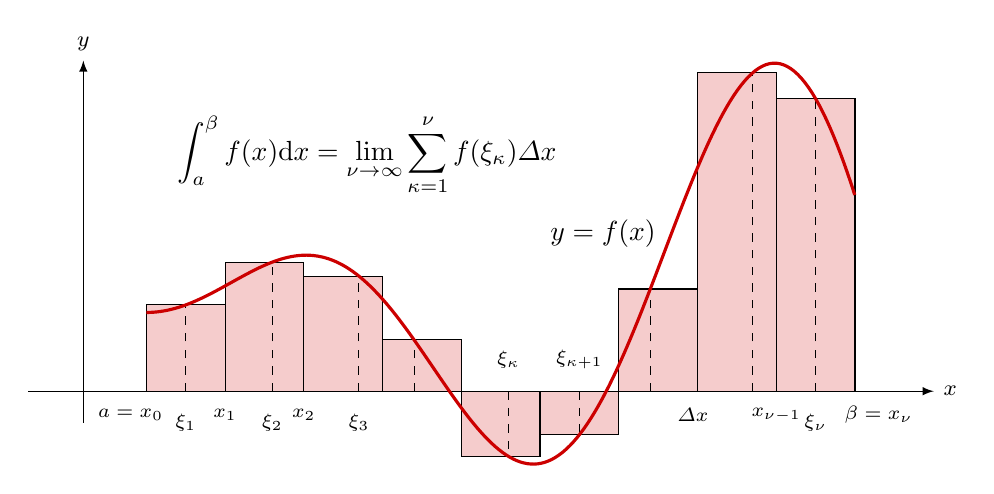
\begin{tikzpicture}[domain=0:9,x=1cm,y=2cm]
\tkzInit[xmin=-1,xmax=7,ymin=-.5,ymax=1.2,ystep=1]
\draw[-latex] (-1.5,0) -- coordinate (x axis mid) (10,0) node[right,fill=white] {{\footnotesize $ x $}};
\draw[-latex] (-.8,-.2) -- (-.8,2.1) node[above,fill=white] {{\footnotesize $ y $}};

\foreach \x/\y in {.5/0,1.6/1,2.7/2,3.4/3,4.6/4,5.5/5,6.4/6,7.7/7,8.5/8}{
\foreach \t in \y{
\draw[fill=\xrwma!20] (\y,0) rectangle (\y+1,{\x*sin(\x r)/5+.5});
\draw[dashed] (\x,0)--(\x,{\x*sin(\x r)/5+.5});}}
\foreach \x/\y in {0.5/1,1.6/2,2.7/3,8.5/\nu}{
\node at (\x,-.2) {\scriptsize $ \xi_\y $};}
\node at (4.6,.2) {\scriptsize $\xi_\kappa $};
\node at (5.5,.2) {\scriptsize $\xi_{\kappa+1} $};
\node at (-.2,-.15) {\scriptsize $ a=x_0 $};
\node at (1,-.15) {\scriptsize $ x_1 $};
\node at (2,-.15) {\scriptsize $ x_2 $};
\node at (9.3,-.15) {\scriptsize $ \beta=x_\nu $};
\node at (8,-.15) {\scriptsize $ x_{\nu-1} $};
\node at (5.8,1) {$  y=f(x) $};
\node at (2.8,1.5) {$  \displaystyle{\int_{a}^{\beta}f(x)\mathrm{d}x=\lim_{\nu\rightarrow\infty}\PARENS{\sum_{\kappa=1}^{\nu}f(\xi_\kappa)\varDelta x} }$};
\draw[samples=200,line width=.4mm,\xrwma] plot ({\x},{\x*sin(deg(\x))/5+.5});
\tkzText(6.5,-.15){$ \undercbrace{\rule{9mm}{0mm}}_{\varDelta x} $}
\end{tikzpicture}\\
\vspace*{\fill}
Φρόνιμος Σπύρος
\end{center}
\pagenumbering{gobble}
\newpage
\null
\newpage
\pagestyle{fancy}
\pagenumbering{arabic}

\newpage
\renewcommand{\myleftmark}{{\large Τυπολόγιο}}
\begin{center}
\part{Τυπολόγιο}
\end{center}
\section{Όρια - Συνέχεια}
\part{Βασικές ασκήσεις}
\section{Όρια - Συνέχεια}
\subsection{Σύνθεση συναρτήσεων}
\begin{askhsh}{Εύρεση σύνθεσης}
Για να οριστεί η συνάρτηση $ f\circ g $ πρέπει να βρούμε το πεδίο ορισμού της και τον τύπο της.\\
\bhmata
\begin{bhma}
\item Ο τύπος της $ f\circ g $ θα ισούται με
\[ (f\circ g)(x)=f(g(x)) \]
που σημαίνει ότι στον τύπο της $ f $ αντικαθιστούμε το $ x $ με $ g(x) $.
\item Για το πεδίο ορισμού ισχύουν οι σχέσεις
\[ x\in D_g\ \ \textrm{ και }\ \ g(x)\in D_f \]
Οι περιορισμοί αυτοί μας οδηγούν σε εξισώσεις και ανισώσεις. Οι κοινές λύσεις σχηματίζουν το πεδίο ορισμού.
\end{bhma}
Εντελώς ανάλογα εργαζόμαστε για τις συναρτήσεις $ g\circ f, f\circ f\ldots $
\end{askhsh}
\Paradeigma{Σύνθεση συναρτήσεων}
\bmath{Δίνονται οι συναρτήσεις $f(x)=\dfrac{1}{x-1}$ και $g(x)=\sqrt{x-2}$. Να ορίσετε τις συναρτήσεις
\begin{multicols}{3}
\begin{alist}
\item $f\circ g$
\item $g\circ f$
\item $f\circ f$
\end{alist}
\end{multicols}}
\lysh
Η συνάρτηση $f$ ορίζεται όταν $x-1\neq 0\Rightarrow x\neq 1$ άρα $D_f=\mathbb{R}-\{1\}$, ενώ η $g$ ορίζεται όταν $x-2\geq 0\Rightarrow x\geq 2$ οπότε $D_g=[2,+\infty)$.
\begin{alist}
\item Η συνάρτηση $f\circ g$ έχει τύπο
\[(f\circ g)(x)=f\left(g(x)\right)=\frac{1}{g(x)-1}=\frac{1}{\sqrt{x-2}-1}\]
και πεδίο ορισμού
\[ D_{f\circ g}=\{x\in D_g\ \text{και}\ g(x)\in D_f\} \]
\begin{itemize}
\item $x\in D_g\Rightarrow x\in [2,+\infty)$
\item $g(x)\in D_f\Rightarrow \sqrt{x-2}\in\mathbb{R}-\{1\}\Rightarrow \sqrt{x-2}\neq 1\Rightarrow x-2\neq 1\Rightarrow x\neq 3$
\end{itemize}
Επομένως $D_{f\circ g}=[2,3)\cup(3,+\infty)$.

\item Η συνάρτηση $g\circ f$ έχει τύπο
\[(g\circ f)(x)=g\left(f(x)\right)=\sqrt{f(x)-2}=\sqrt{\frac{1}{x-1}-2}\]
και πεδίο ορισμού
\[ D_{g\circ f}=\{x\in D_f\ \text{και}\ f(x)\in D_g\} \]
\wrapr{-15mm}{7}{6cm}{4mm}{
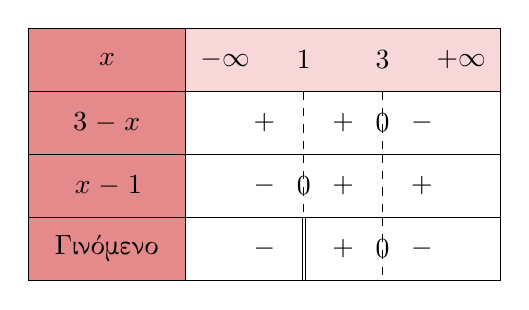
\begin{tikzpicture}
\tikzset{t style/.style = {style = dashed}}
\tikzset{z style/.style = {fill=white,inner sep=.2mm}}
\tkzTabInit[color,lgt=2,espcl=1,colorC = red7,
colorL = red9,
colorV = red7]%
{$x$ / .8,$3-x$ /0.8,$x-1$/0.8, Γινόμενο/0.8}%
{$-\infty$,$1$,$3$,$+\infty$}%
\tkzTabLine{ , +, t, +,z ,- , }
\tkzTabLine{ , -, z, +,t ,+ , }
\tkzTabLine{ , -, d, +,z ,- , }
\end{tikzpicture}
}{
\begin{itemize}
\item $x\in D_f\Rightarrow x\in\mathbb{R}-\{1\}$
\item 
$\begin{aligned}[t]
f(x)\in D_g&\Rightarrow \dfrac{1}{x-2}\in[2,+\infty)\Rightarrow \dfrac{1}{x-1}\geq 2\Rightarrow\\&\Rightarrow\dfrac{1}{x-1}-2\geq 0\Rightarrow\dfrac{3-x}{x-1}\geq 0\Rightarrow\\&\Rightarrow (3-x)(x-1)\geq 0\ \text{και}\ x-1\neq 0\Rightarrow\\
&\Rightarrow x\in(1,3]
\end{aligned}$
\end{itemize}}
Επομένως $D_{g\circ f}=(1,3]$.
\end{alist}
\subsection{Συνάρτηση \bmath{$ 1-1 $} - Αντίστροφη}
\begin{askhsh}{Συνάρτηση $ 1-1 $}
\tropoi\begin{tropos}
\item Αποδεικνύουμε ότι η $ f $ είναι γνησίως μονότονη στο $ D_f $. (Ο τρόπος αυτός ενδείκνυται όταν το πεδίο ορισμού της $ f $ είναι ένα διάστημα.)
\item Με τη βοήθεια του ορισμού της $ 1-1 $ συνάρτησης
\[ \textrm{Για κάθε }x_1,x_2\in D_f \ \ : \ \  f(x_1)=f(x_2)\Rightarrow x_1=x_2 \]
(Ο τρόπος αυτός ενδείκνυται για συναρτήσεις με πεδίο ορισμού ένωση διαστημάτων, αρκεί ο τύπος να επιτρέπει την επίλυση της εξίσωσης.)
\item Με τη βοήθεια της γραφικής παράστασης της $ f $. Κάθε οριζόντια ευθεία πρέπει να τέμνει τη $ C_f $ σε ένα το πολύ σημείο.
\item Αν η εξίσωση $ y=f(x) $ έχει μοναδική λύση ως προς $ x $ για κάθε $ y\in f(D_f) $ και η λύση ανήκει στο $ D_f $ τότε η $ f $ είναι $ 1-1 $.
\item Με απαγωγή σε άτοπο. Υποθέτουμε δηλαδή ότι η $ f $ δεν είναι $ 1-1 $.
\end{tropos}
\end{askhsh}
\begin{askhsh}{Εύρεση αντίστροφης συνάρτησης}
\bhmata\begin{bhma}
\item Δείχνουμε ότι η $f$ είναι $1-1$.
\item Εύρεση συνόλου τιμών της $ f $ με τη βοήθεια μονοτονίας.
\item Επίλυση της εξίσωσης $ y=f(x) $ ως προς $ x $ με $ x\in D_f $.
\end{bhma}
\end{askhsh}
\Paradeigma{Εύρεση αντίστροφης}
\bmath{Δίνεται η συνάρτηση $f(x)=\ln{(x-2)-\ln{(5-x)}}$. Να δείξετε ότι η $f$ είναι αντιστρέψιμη και να ορίσετε τη συνάρτηση $f^{-1}$.}\\\\
\lysh
Η $f$ ορίζεται όταν
\[
x-2>0\Rightarrow x>2\ \text{και}\ 5-x>0\Rightarrow x<5
\]
άρα $D_f=(2,5)$. Για κάθε $x\in(2,5)$ είναι:
\[ f'(x)=\left[\ln{(x-2)-\ln{(5-x)}}\right]'=\frac{(x-2)'}{x-2}-\frac{(5-x)'}{5-x}=\frac{1}{x-2}+\frac{1}{5-x}>0 \]
επομένως η $f$ είναι γνησίως αύξουσα στο $(2,5)$, άρα και $1-1$ οπότε αντιστρέφεται. Η $f^{-1}$ έχει πεδίο ορισμού
\[ D_{f^{-1}}=f(D_f)=f((2,5))\stackrel{f\nearrow}{=}\left(\lim\limits_{x\to2^+}{f(x)},\lim\limits_{x\to5^-}{f(x)}\right) \]
\begin{itemize}
\item $\lim\limits_{x\to2^+}{f(x)}=\lim\limits_{x\to2^+}{\left(\ln{(x-2)}-\ln{(5-x)}\right)}=-\infty-\ln{3}=-\infty$.
\item $\lim\limits_{x\to5^-}{f(x)}=\lim\limits_{x\to5^-}{\left(\ln{(x-2)}-\ln{(5-x)}\right)}=\ln{3}-(-\infty)=+\infty$.
\end{itemize}
οπότε $D_{f^{-1}}=\mathbb{R}$. Για την εύρεση του τύπου έχουμε $y=f(x)\Leftrightarrow x=f^{-1}(y)$. Είναι λοιπόν
\begin{align*}
y=f(x)&\Leftrightarrow y=\ln{(x-2)}-\ln{(5-x)}\Leftrightarrow y=\ln{\frac{x-2}{5-x}}\Leftrightarrow\\
&\Leftrightarrow e^y=\frac{x-2}{5-x}\Leftrightarrow e^y(5-x)=x-2\Leftrightarrow\\
&\Leftrightarrow 5e^y-xe^y=x-2\Leftrightarrow x+xe^y=5e^y+2\Leftrightarrow\\
&\Leftrightarrow x\left(e^y+1\right)=5e^y+2\Leftrightarrow x=\frac{5e^y+2}{e^y+1}\Leftrightarrow f^{-1}(y)=\frac{5e^y+2}{e^y+1}
\end{align*}
άρα η αντίστροφη της $f$ είναι $f^{-1}(x)=\frac{5e^x+2}{e^x+1}\ ,\ D_{f^{-1}}=\mathbb{R}$.
\subsection{Όρια μορφής \bmath{$\frac{0}{0}$}}
\begin{askhsh}{Όριο $ \frac{0}{0} $ ρητής}
Αν ένα όριο $\lim\limits_{x\to x_0}{\frac{P(x)}{Q(x)}}$, όπου $P(x),Q(x)$ πολυώνυμα, έχει μορφή $\frac{0}{0}$ τότε εργαζόμαστε ως εξής:
\begin{tropos}
\item \kerkissans{\textbf{Παραγοντοποίηση}}
\\\bhmata\begin{bhma}
\item Παραγοντοποιούμε αριθμητή και παρονομαστή.
\item Απλοποιούμε τις παραστάσεις $x-x_0$ και αντικαθιστούμε όπου $x$ το $x_0$.
\end{bhma}
\item \kerkissans{\textbf{Κανόνας \en{De L'Hospital}}}\\
Εφαρμόζουμε τον κανόνα \en{De L'Hospital} όσες φορές χρειαστεί έως ότου φύγει η απροσδιοριστία.
\end{tropos}
\end{askhsh}
\Paradeigma{Όριο $\frac{0}{0}$ ρητής - Παραγοντοποίηση}
\bmath{Υπολογίστε τα παρακάτω όρια
\begin{multicols}{4}
\begin{alist}
\item $\lim\limits_{x\to 2}{\dfrac{x^2-4}{x^2-2x}}$
\item $\lim\limits_{x\to -1}{\dfrac{x^2-x-2}{x^3+1}}$
\item $\lim\limits_{x\to 1}{\dfrac{x^3-7x+6}{x-x^2}}$
\item $\lim\limits_{x\to \frac{1}{2}}{\dfrac{4x^2-4x+1}{4x^2-1}}$
\end{alist}
\end{multicols}}
\lysh
\Paradeigma{Όριο $\frac{0}{0}$ ρητής - Κανόνας \en{De L'Hospital}}
\bmath{Υπολογίστε τα παρακάτω όρια
\begin{multicols}{2}
\begin{alist}
\item $\lim\limits_{x\to 2}{\dfrac{x^2+3x-10}{x^3-8}}$
\item $\lim\limits_{x\to -1}{\dfrac{x^2+2x+1}{x^2-x}}$
\end{alist}
\end{multicols}}
\lysh
\begin{askhsh}{Όριο $ \frac{0}{0} $ άρρητης}
Πολλαπλασιασμός με συζυγείς παραστάσεις.
\end{askhsh}
\Paradeigma{Όριο $\frac{0}{0}$ άρρητης}
\bmath{Υπολογίστε τα παρακάτω όρια
\begin{multicols}{2}
\begin{alist}
\item $\lim\limits_{x\to 2}{\dfrac{\sqrt{3x-2}-2}{x^2-4}}$
\item $\lim\limits_{x\to 2}{\dfrac{\sqrt{x+1}-\sqrt{2x-1}}{\sqrt{x+2}-2}}$
\end{alist}
\end{multicols}}
\begin{askhsh}{Όριο $ \frac{0}{0} $ ρητής με απόλυτες τιμές}
\bhmata\begin{bhma}
\item Υπολογίζω τα όρια των παραστάσεων μέσα στις απόλυτες τιμές.
\item Διώχνω τις απόλυτες τιμές με τον παρακάτω κανόνα
\begin{gather*}
\lim_{x\to x_0}{f(x)}>0\Rightarrow f(x)>0\ \textrm{κοντά στο }x_0\\
\lim\limits_{x\to x_0}{f(x)}<0\Rightarrow f(x)<0\  \textrm{κοντά στο }x_0
\end{gather*}
Αν κάποια απόλυτη τιμή μηδενίζεται στο $ x_0 $ τότε υπολογίζω πλευρικά όρια.
\item Υπολογίζω όριο ρητής $ \frac{0}{0} $
\end{bhma}
\end{askhsh}
\begin{askhsh}{Όριο $ \frac{0}{0} $ με τριγωνομετρικές παραστάσεις}
\begin{tropos}
\item Κατασκευάζω και χρησιμοποιώ τριγωνομετρικές ταυτότητες.
\item Κατασκευάζω με πράξεις κάποιο βασικό τριγωνομετρικό όριο, αρκεί όταν $ x\to x_0 $ να μηδενίζεται η γωνία του τριγωνομετρικού αριθμού.
\item Κανόνας \en{De L' Hospital}. (Χρειάζεται προσοχή εδώ γιατί μπορεί η εφαρμογή του κανόνα να με οδηγήσει σε δυσκολότερο όριο.)
\end{tropos}
\end{askhsh}
\begin{askhsh}{Όριο $ \frac{0}{0} $ με εκθετικές, λογαριθμικές και συνδυασμό αυτών}
Εφαρμογή του κανόνα \eng{De L' Hospital}.
\end{askhsh}
\subsection{{Όρια με απροσδιοριστία $ \frac{\pm\infty}{\pm\infty} $}}
\begin{askhsh}{Όρια $ \frac{\pm\infty}{\pm\infty} $ ρητής}
Με ρητή συνάρτηση όταν $ x\to\pm\infty $ υπολογίζουμε το όριο του κλάσματος μόνο με τους μεγιστοβάθμιους όρους.
\end{askhsh}
\begin{askhsh}{Όρια $ \frac{\pm\infty}{\pm\infty} $ με ρίζες}
Μέθοδος κοινού παράγοντα ή συζυγείς παραστάσεις.
\end{askhsh}
\begin{askhsh}{Όρια $ \frac{\pm\infty}{\pm\infty} $ Διάφορες συναρτήσεις}
 Κανόνας \en{De L' Hospital}
\end{askhsh}
\subsection{Όρια με απροσδιοριστία \bmath{$ 0\cdot(\pm\infty) $}}
\begin{askhsh}{Όρια $ 0\cdot(\pm\infty) $ - Γενική μέθοδος}
\bhmata\begin{bhma}
\item Γράφουμε το γινόμενο με μορφή σύνθετου κλάσματος ως εξής
\[ \lim_{x\to x_0}{\left(f(x)\cdot g(x)\right)}=\lim_{x\to x_0}{\dfrac{f(x)}{\frac{1}{g(x)}}}\ \ \textrm{ή}\ \ \lim_{x\to x_0}{\dfrac{g(x)}{\frac{1}{f(x)}}} \]
\item Το όριο παίρνει τη μορφή $ \dfrac{0}{0} $ ή $ \dfrac{\pm\infty}{\pm\infty} $ οπότε εφαρμόζουμε κανόνα \en{De L' Hospital}
\end{bhma}
\end{askhsh}
\begin{askhsh}{Όρια με απροσδιοριστία $ 0^0,1^{\pm\infty},(\pm\infty)^0 $}
\bhmata\begin{bhma}
\item Χρησιμοποιούμε τον παρακάτω κανόνα
\[ \lim_{x\to x_0}{f(x)^{g(x)}}=\lim_{x\to x_0}{e^{\ln{f(x)^{g(x)}}}}=\lim_{x\to x_0}{e^{g(x)\cdot\ln{f(x)}}} \]
\item Υπολογίζουμε το όριο του εκθέτη το οποίο έχει απροσδιοριστία $ 0\cdot(\pm\infty) $. Στη συνέχεια με αντικατάσταση υπολογίζουμε το αρχικό όριο.
\end{bhma}
\end{askhsh}
\subsection{Όρια με απροσδιοριστία \bmath{$ +\infty-\infty $}}
\begin{askhsh}{Όρια $ +\infty-\infty $ - Γενική μέθοδος}
\bhmata
\begin{bhma}
\item Βγάζουμε κοινό παράγοντα μια από τις δύο συναρτήσεις.
\[ \lim_{x\to x_0}{(f(x)-g(x))}=\lim_{x\to x_0}{\left[f(x)\left(1-\frac{g(x)}{f(x)}\right)\right]} \]
\item Στη συνέχεια υπολογίζουμε το όριο του κλάσματος $ \frac{g(x)}{f(x)} $ με μορφή $ \frac{\pm\infty}{\pm\infty} $.
\item Επιστρέφουμε στο αρχικό όριο αντικαθιστώντας.
\end{bhma}
\end{askhsh}
\begin{askhsh}{Όρια $ +\infty-\infty $ - Κλάσματα}
Αν στο όριο $\lim_{x\to x_0}{(f(x)-g(x))}$ οι συναρτήσεις $ f(x),g(x) $ είναι κλάσματα τότε τα κάνουμε ομώνυμα και οδηγούμαστε σε μία από τις μορφές $\frac{0}{0}$,$\frac{\pm\infty}{\pm\infty}$ ή $\frac{a}{0}$.
\end{askhsh}
\begin{askhsh}{Όρια $ +\infty-\infty $ - Διαφορά λογαρίθμων}
Σχηματίζουμε διαφορά λογαρίθμων και χρησιμοποιούμε την ιδιότητα
\[ \ln{a}-\ln{\beta}=\ln{\frac{a}{\beta}} \]
Στη συνέχεια υπολογίζουμε το όριο του κλάσματος το οποίο έχει απροσδιοριστία $\frac{\pm\infty}{\pm\infty}$.
\end{askhsh}
\begin{askhsh}{Όρια της μορφής $ \frac{a}{0} $}
\bhmata\begin{bhma}
\item Παραγοντοποιούμε τον παρονομαστή.
\item Γράφουμε σε ξεχωριστό κλάσμα τον παράγοντα που μηδενίζεται.
\item Αν αυτός ο παράγοντας έχει σταθερό πρόσημο τότε προχωράμε στον υπολογισμό. Αν όχι υπολογίζουμε πλευρικά όρια.
\end{bhma}
\end{askhsh}
\begin{askhsh}{Όρια με τριγωνομετρικές συναρτήσεις $ \hm{f(x)},\syn{f(x)} $ - Μηδενική επί φραγμένη}
Αν το όριο περιέχει σύνθετες τριγωνομετρικές συναρτήσεις με γωνία $ f(x) $ και $ \lim\limits_{x\to x_0}{f(x)}=\pm\infty $ τότε
\\\bhmata\begin{bhma}
\item Γράφουμε τη συνάρτηση μέσα στο όριο ως γινόμενο συναρτήσεων. 
\item Κλείνουμε τη συνάρτηση του ορίου σε απόλυτη τιμή και σχηματίζουμε διπλή ανισότητα ώστε να εφαρμοστεί κριτήριο παρεμβολής.
\end{bhma}
\end{askhsh}
\begin{askhsh}{Γνωστό όριο που περιέχει την $ f(x) $ - Βοηθητική συνάρτηση}
\bhmata\begin{bhma}
\item Θέτουμε $ g(x) $ τη συνάρτηση του ορίου και λύνουμε ως προς $ f(x) $.
\item Υπολογίζουμε το όριο της $ f $ στο $ x_0 $.
\end{bhma}
\end{askhsh}
\begin{askhsh}{Κριτήριο παρεμβολής}
Το κριτήριο παρεμβολής για τον υπολογισμό ορίων εφαρμόζεται σε ανισότητες της μορφής
\[ g(x)\leq f(x)\leq h(x)\ \ \textrm{ή}\ \ |f(x)|\leq g(x)\Rightarrow -g(x)\leq f(x)\leq g(x) \]
\end{askhsh}
\section{Διαφορικός λογισμός}
\subsection{Εφαπτομένη}
\begin{askhsh}{Εύρεση εφαπτομένης με γνωστό σημείο επαφής}
\bhmata\begin{bhma}
\item Πεδίο ορισμού, παράγωγος $ f' $ και θέτουμε όπου $ x=x_0 $ ώστε να βρεθούν οι αριθμοί $ f(x_0) $ και $ f'(x_0) $.
\item Γράφουμε την εξίσωση της ευθείας
\[ y-f(x_0)=f'(x_0)(x-x_0) \]
και αντικαθιστώντας λύνουμε ως προς $ y $.
\end{bhma}
\end{askhsh}
\Paradeigma{Εφαπτομένη - Γνωστό σημείο επαφής}
\bmath{Δίνεται η συνάρτηση $f(x)=\frac{e^x}{x-1}$. Να βρεθεί η εξίσωση της εφαπτόμενης ευθείας της $C_f$ στο σημείο
\begin{multicols}{2}
\begin{alist}
\item $M(0,f(0))$
\item με τεταγμένη $e^2$.
\end{alist}
\end{multicols}}
\begin{askhsh}{Εύρεση εφαπτομένης με γνωστή κλίση λ}
\bhmata\begin{bhma}
\item Πεδίο ορισμού και $ f' $.
\item Θεωρούμε σημείο επαφής $ M(x_0,f(x_0)) $ και θέτουμε το σ.δ. της εφαπτομένης να ισούται με τη δοσμένη κλίση $ \lambda $.
\[ f(x_0)=\lambda \]
Αν δεν μας δίνεται ο συντελεστής $ \lambda $ της εφαπτομένης $ \varepsilon $ τότε τον βρίσκουμε έχοντας τις εξής περιπτώσεις.
\begin{center}
\begin{mytblr}{cc}
\textbf{Συνθήκη} & \textbf{Εξίσωση} \\
Ευθείες παράλληλες $ \varepsilon\parallel \zeta $ &$ \lambda_{\varepsilon}=\lambda_{\zeta}\Rightarrow f'(x_0)=\lambda $  \\
Ευθείες κάθετες $ \varepsilon\perp\zeta $ & $ \lambda_{\varepsilon}\cdot\lambda_{\zeta}=-1\Rightarrow \ldots\Rightarrow f'(x_0)=\lambda $ \\
Οριζόντια ευθεία $ \varepsilon\parallel x'x $  & $ \lambda_{\varepsilon}=0\Rightarrow f'(x_0)=0 $ \\
Η $ \varepsilon $ σχηματίζει γωνία $ \omega $ & $ \lambda_{\varepsilon}=\ef{\omega}\Rightarrow f'(x_0)=\ef{\omega} $.
\end{mytblr}
\end{center}
\item Λύνουμε την εξίσωση, βρίσκουμε το $ x_0 $ και στη συνέχεια το $ f(x_0) $.
\item Εξίσωση ευθείας $ y-f(x_0)=f'(x_0)(x-x_0) $.
\end{bhma}
\end{askhsh}
\begin{askhsh}{Εφαπτομένη που διέρχεται από εξωτερικό σημείο $ P(a,\beta) $}
\bhmata\begin{bhma}
\item Πεδίο ορισμού και $ f' $.
\item Θεωρούμε σημείο επαφής $ M(x_0,f(x_0)) $ και γράφουμε τον τύπο της ευθείας.
\item Αντικαθιστούμε $ f(x_0) $ και $ f'(x_0) $ στην εξίσωση.
\item Αφού $ P\in\varepsilon $ τότε θέτουμε $ x=a $ και $ y=\beta $ και λύνουμε την εξίσωση ως προς $ x_0 $.
\item Για κάθε $ x_0 $ υπολογίζουμε $ f(x_0) $ και $ f'(x_0) $ και βρίσκουμε την ευθεία.
\end{bhma}
\end{askhsh}
\begin{askhsh}{Ευθεία εφάπτεται στη $ C_f $ στο $ M(x_0f(x_0)) $}
\[ \textrm{Η ευθεία }y=ax+\beta\textrm{ εφάπτεται στη }C_f\Leftrightarrow \ccases{f(x_0)=ax_0+\beta\\f'(x_0)=a} \]
\end{askhsh}
\begin{askhsh}{Κοινή εφαπτομένη $ C_f,C_g $ σε κοινό σημείο $ M(x_0,f(x_0)) $}
\[ \textrm{Οι }C_f\textrm{ και }C_g\textrm{ έχουν κοινή εφαπτομένη στο }Μ\Leftrightarrow \ccases{f(x_0)=g(x_0)\\f'(x_0)=g'(x_0)} \]
\end{askhsh}


\subsection{Μονοτονία - Ακρότατα}
\begin{askhsh}{Μονοτονία - Ακρότατα - Σύνολο τιμών - Πλήθος ριζών}
\bhmata\begin{bhma}
\item Πεδίο ορισμού της $ f $ και έλεγχος συνέχειας.
\item Παράγωγος $ f' $.
\item Υπολογίζουμε τις ρίζες και τα πρόσημα της $ f' $ με έναν από τους παρακάτω τρόπους :
\begin{itemize}[leftmargin=5mm]
\item Λύνοντας την εξίσωση $ f(x)=0 $  και τις ανισώσεις $ f(x)>0 $ και $ f(x)<0 $.
\item Με επιλογή τιμής σε κάθε διάστημα που χωρίζουν οι ρίζες το πεδίο ορισμού.
\item Παραγωγίζοντας δεύτερη ή ακόμα και τρίτη φορά. Με τη μονοτονία κάθε παραγώγου βρίσκουμε τα πρόσημά της ώσπου να φτάσουμε στη μονοτονία της $ f $. Οι ρίζες βρίσκονται με δοκιμές.
\end{itemize}
\item Πίνακας μονοτονίας και ακροτάτων.
\item Μονοτονία - Ακρότατα - Σύνολο τιμών - Πλήθος ριζών\\\vspace{-7mm}
\begin{itemize}[leftmargin=5mm]
\item \textbf{Για εύρεση μονοτονίας} αναφέρουμε το είδος της μονοτονίας σε κάθε διάστημα ξεχωριστά. 
\item \textbf{Για εύρεση ακροτάτων} ελέγχουμε για ακρότατα στα κρίσιμα σημεία και στα κλειστά άκρα του πεδίου ορισμού 
\item \textbf{Για εύρεση συνόλου τιμών} βρίσκουμε τις εικόνες των διαστημάτων μονοτονίας και τις ενώνουμε.
\item \textbf{Για την εύρεση του πλήθους ριζών της συνάρτησης} ελέγχουμε αν το $ 0 $ ανήκει στην εικόνα κάθε διαστήματος. Αναλυτικά
\[ 0\in f(\Delta_1)\Rightarrow \textrm{Υπάρχει }x_0 : f(x_0)=0 \]
Η ρίζα αυτή είναι μοναδική μέσα στο κάθε διάστημα γιατί η $ f $ είναι γνησίως μονότονη.
\end{itemize}
\end{bhma}
\end{askhsh}
\Paradeigma{Μονοτονία - Ακρότατα - Σύνολο τιμών - Πλήθος ριζών}
\bmath{Δίνεται η συνάρτηση $f:\mathbb{R}^*\to\mathbb{R}$ με τύπο $f(x)=x+\dfrac{1}{x}$. Να βρείτε
\begin{multicols}{2}
\begin{alist}
\item τα διαστήματα μονοτονίας της $f$.
\item τα τοπικά ακρότατα.
\item το σύνολο τιμών της $f$.
\item το πλήθος ριζών της εξίσωσης $f(x)=3$.
\end{alist}
\end{multicols}}
\lysh
Για κάθε $x\neq 0$ έχουμε:
\[ f'(x)=\left(x+\frac{1}{x}\right)'=1-\frac{1}{x^2}-\frac{x^2-1}{x^2} \]
\begin{itemize}
\item $f'(x)=0\Rightarrow \frac{x^2-1}{x^2}=0\Rightarrow x^2-1=0\Rightarrow x^2=1\Rightarrow x=\pm 1$
\item $f'(x)>0\Rightarrow \frac{x^2-1}{x^2}>0\xRightarrow{x^2>0} x^2-1>0\Rightarrow x^2>1\Rightarrow |x|>1\Rightarrow x\in(-\infty,-1)\cup(1,\infty)$.
\item $f'(x)<0\Rightarrow \frac{x^2-1}{x^2}<0\xRightarrow{x^2>0} x^2-1<0\Rightarrow x^2<1\Rightarrow |x|<1\Rightarrow x\in(-1,1)$.
\end{itemize}
Στον παρακάτω πίνακα βλέπουμε τα πρόσημα της $f'$ και τη μονοτονίας της $f$.\\
\wrapl{-10mm}{5}{6.4cm}{0mm}{
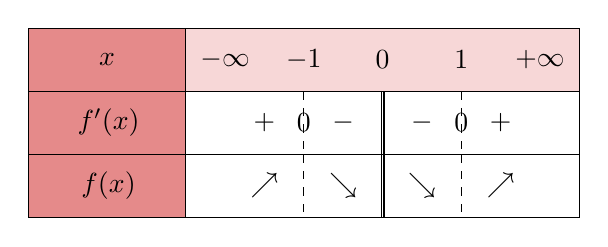
\begin{tikzpicture}
\tikzset{t style/.style = {style = dashed}}
\tikzset{z style/.style = {fill=white,inner sep=.2mm}}
\tkzTabInit[color,lgt=2,espcl=1,colorC = red7,
colorL = red9,
colorV = red7]%
{$x$ / .8,$f'(x)$ /0.8,$f(x)$/0.8}%
{$-\infty$,$-1$,$0$,$1$,$+\infty$}%
\tkzTabLine{ , +, z,-,d, -,z ,+, }
\tkzTabLine{ , \nearrow , t , \searrow,d , \searrow  , t, \nearrow ,}
\end{tikzpicture}
}{\begin{alist}
\item Η $f$ είναι γνησίως αύξουσα στ διαστήματα $(-\infty,-1]$ και $[1,+\infty)$ και γνησίως φθίνουσα στο $[-1,1]$.
\item Η $f$ παρουσιάζει τοπικό μέγιστο στη θέση $x=-1$, το $f(-1)=-2$ και τοπικό ελάχιστο στη θέση $x=1$, το $f(1)=2$.
\end{alist}}\\
\begin{alist}[resume]
\item Η $f$ είναι γνησίως αύξουσα στο $\varDelta_1=(-\infty,-1]$ άρα $f(\varDelta_1)=\left(\lim\limits_{x\to-\infty}{f(x)},f(-1)\right]=(-\infty,-2]$ αφού
\[ \lim_{x\to -\infty}{f(x)}=\lim_{x\to-\infty}{\left(x+\frac{1}{x}\right)}=-\infty+0=-\infty \]
Επίσης η $f$ είναι γνησίως φθίνουσα στο $\varDelta_2=[-1,0)$ άρα $f(\varDelta_2)=\left(\lim\limits_{x\to0^-}{f(x)},f(-1)\right]=(-\infty,-2]$ αφού
\[ \lim_{x\to0^-}{f(x)}=\lim_{x\to0^-}{\left(x+\frac{1}{x}\right)}=0-\infty=-\infty \]
Ομοίως, για $\varDelta_3=(0,1]$ και $\varDelta_4=[1,+\infty)$, προκύπτουν $f(\varDelta_3)=f(\varDelta_4)=[2,+\infty)$. Επομένως η $f$ έχει σύνολο τιμών
\[f(D_f)=f(\varDelta_1)\cup f(\varDelta_2)\cup f(\varDelta_3)\cup f(\varDelta_4)=(-\infty,-2]\cup[2,+\infty).\]
\item Για την εξίσωση $f(x)=3$ παρατηρούμε ότι 
\begin{itemize}
\item $3\notin f(\varDelta_1)$ άρα η εξίσωση δεν έχει ρίζα στο $\varDelta_1$.
\item $3\notin f(\varDelta_2)$ άρα η εξίσωση δεν έχει ρίζα στο $\varDelta_1$.
\item $3\in f(\varDelta_3)$ άρα η εξίσωση έχει τουλάχιστον 1 ρίζα στο $\varDelta_3$ η οποία είναι μοναδική αφού $f\searrow\varDelta_3$.
\item $3\in f(\varDelta_4)$ άρα η εξίσωση έχει τουλάχιστον 1 ρίζα στο $\varDelta_4$ η οποία είναι μοναδική αφού $f\nearrow\varDelta_4$.
\end{itemize}
Οπότε η εξίσωση έχει ακριβώς $2$ ρίζες.
\end{alist}
\subsection{Κυρτότητα και σημεία καμπής}
\begin{askhsh}{Εύρεση κυρτότητας - σημείων καμπής}
\bhmata\begin{bhma}
\item Πεδίο ορισμού και έλεγχος συνέχειας.
\item Υπολογίζουμε την δεύτερη παράγωγο $ f'' $.
\item Βρίσκουμε ρίζες και πρόσημα της $ f'' $ με τους τρόπους που περιγράψαμε στη μονοτονία.
\item Σχηματίζουμε πίνακα με τα πρόσημα της $ f'' $ και την κυρτότητα της $ f $.
\item Κυρτότητα - Σημεία καμπής\\\vspace{-7mm}
\begin{itemize}[leftmargin=5mm]
\item \textbf{Για εύρεση κυρτότητας} αναφέρουμε το είδος της κυρτότητας σε κάθε διάστημα ξεχωριστά.
\item \textbf{Για εύρεση σημείων καμπής} ελέγχουμε για σημεία καμπής στα σημεία που αλλάζει η κυρτότητα αρκεί η $ f $ να είναι μια φορά παραγωγίσιμη στα σημεία αυτά.
\end{itemize}
\end{bhma}
\end{askhsh}
\noindent
\Paradeigma{Δίνεται η συνάρτηση $f(x)=\frac{2x}{x^2+1}$. Μελετήστε την συνάρτηση $f$ ως προς την κυρτότητα και τα σημεία καμπής.}\\
\lysh
Η συνάρτηση $f$ ορίζεται στο $D_f=\mathbb{R}$ καθώς $x^2+1\neq 0$ για κάθε $x\in\mathbb{R}$ και είναι συνεχής ως ρητή. Για κάθε $x\in\mathbb{R}$ είναι
\begin{align*}
f'(x)&=\left(\frac{2x}{x^2+1}\right)'=\frac{(2x)'\left(x^2+1\right)-2x\left(x^2+1\right)'}{\left(x^2+1\right)^2}=\\
&=\frac{2\left(x^2+1\right)-2x\cdot 2x}{\left(x^2+1\right)^2}=\frac{2x^2+2-4x^2}{\left(x^2+1\right)^2}=\frac{2-2x^2}{\left(x^2+1\right)^2}\ \ \text{ και}\\
f''(x)&=\left[\frac{2-2x^2}{\left(x^2+1\right)^2}\right]'=\frac{\left(2-2x^2\right)'\left(x^2+1\right)^2-\left(2-2x^2\right)\left[\left(x^2+1\right)^2\right]'}{\left(x^2+1\right)^4}=\\&=\frac{-4x\left(x^2+1\right)^2-\left(2-2x^2\right)2\left(x^2+1\right)\left(x^2+1\right)'}{\left(x^2+1\right)^4}=\frac{\left(x^2+1\right)\left[-4x\left(x^2+1\right)-4x\left(2-2x^2\right)\right]}{\left(x^2+1\right)^4}=\\
&=\frac{-4x^3-4x-8x+8x^3}{\left(x^2+1\right)^3}=\frac{4x^3-12x}{\left(x^2+1\right)^3}
\end{align*}
Έχουμε λοιπόν
\begin{itemize}
\item $f''(x)=0\Rightarrow \dfrac{4x^3-12x}{\left(x^2+1\right)^3}=0\Rightarrow 4x^3-12x=0\Rightarrow x=0\ \text{ή}\ x=\pm\sqrt{3}$.
\item $f''(x)>0\Rightarrow \dfrac{4x^3-12x}{\left(x^2+1\right)^3}>0\Rightarrow 4x^3-12x>0\Rightarrow x\in(-\sqrt{3},0)\cup(\sqrt{3},+\infty)$.
\item $f''(x)<0\Rightarrow \dfrac{4x^3-12x}{\left(x^2+1\right)^3}<0\Rightarrow 4x^3-12x<0\Rightarrow x\in(-\infty,-\sqrt{3})\cup(0,\sqrt{3})$.
\end{itemize}
Στον παρακάτω πίνακα βλέπουμε τα πρόσημα της $f''$ καθώς και την κυρτότητα και τα σημεία καμπής της $f$.
\wrapl{0mm}{7}{7cm}{-5mm}{
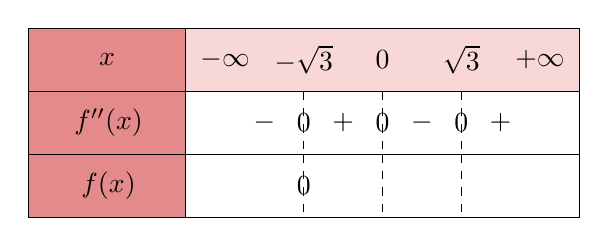
\begin{tikzpicture}
\tikzset{t style/.style = {style = dashed}}
\tikzset{z style/.style = {fill=white,inner sep=.2mm}}
\tkzTabInit[color,lgt=2,espcl=1,colorC = red7,
colorL = red9,
colorV = red7]%
{$x$ / .8,$f''(x)$ /0.8,$f(x)$/0.8}%
{$-\infty$,$-\sqrt{3}$,$0$,$\sqrt{3}$,$+\infty$}%
\tkzTabLine{ , -, z, +,z ,- ,z,+, }
\tkzTabLine{ , \curvearrowright, z, \rotatebox[origin= c]{180}{$\curvearrowleft$},t ,\curvearrowright,t ,\rotatebox[origin= c]{180}{$\curvearrowleft$}, }
\end{tikzpicture}
}{Η συνάρτηση $f$ είναι κυρτή στα διαστήματα $[-\sqrt{3},0]$ και $[\sqrt{3},+\infty)$ και κοίλη στα διαστήματα $(-\infty,-\sqrt{3}]$ και $[0,\sqrt{3}]$. Η $C_f$ έχει σημεία καμπής τα $A(-\sqrt{3},f(-\sqrt{3}))=A\left(-\sqrt{3},-\frac{\sqrt{3}}{2}\right)$, $B(0,f(0))=B(0,0)$ και $\varGamma(\sqrt{3},f(\sqrt{3}))=\varGamma\left(\sqrt{3},\frac{\sqrt{3}}{2}\right)$.}\\
\begin{askhsh}{Κυρτότητα και εφαπτομένες - Απόδειξη ανισότητας}
\bhmata\begin{bhma}
\item Μελετάμε τη συνάρτηση ως προς την κυρτότητα.
\item Βρίσκουμε την εξίσωση της εφαπτομένης στο σημείο που ζητάει ή σε κάποιο σημαντικό σημείο. Αυτή θα έχει τη μορφή $ y=ax+\beta $
\item Χρησιμοποιούμε μια από τις παρακάτω σχέσεις
\[ f\rotatebox[origin=c]{180}{$ \curvearrowleft $}\Delta\Rightarrow f(x)\geq ax+\beta\ \ ,\ \ f\curvearrowright\Delta\Rightarrow f(x)\leq ax+\beta \]
και με πράξεις φέρνουμε την ανισότητα στη μορφή που τη ζητάει η άσκηση.
\end{bhma}
\end{askhsh}

\subsection{Ασύμπτωτες}
\begin{askhsh}{Κατακόρυφες ασύμπτωτες}
\bhmata\begin{bhma}
\item Πεδίο ορισμού της $ f $.
\item Υπολογισμός κάποιου πλευρικού ορίου στα σημεία $ x_0 $ που είναι ανοικτά άκρα του πεδίου ορισμού της $ f $ ή στα σημεία που δεν είναι συνεχής η συνάρτηση.
\item Αν κάποιο πλευρικό όριο ισούται με $ \pm\infty $ τότε η ευθεία $ x=x_0 $ είναι κατακόρυφη ασύμπτωτη της $ C_f $.
\end{bhma}
\end{askhsh}
\begin{askhsh}{Οριζόντια ασύμπτωτη}
\bhmata\begin{bhma}
\item Όριο της $ f $ στο $ +\infty $ ή $ -\infty $ εφόσον ορίζεται η $ f $ σε διάστημα που περιέχει $ \pm\infty $.
\item Αν $ \lim\limits_{x\to \pm\infty}{f(x)}=l $ τότε η ευθεία $ y=l $ είναι οριζόντια ασύμπτωτη της $ C_f $ στο $ \pm\infty $.
\end{bhma}
\end{askhsh}

\begin{askhsh}{Πλάγια ασύμπτωτη}
\bhmata\begin{bhma}
\item Εφόσον ορίζεται η $ f $ σε διάστημα που περιέχει $ \pm\infty $ υπολογίζουμε τα παρακάτω όρια.
\[ \lim_{x\to +\infty}{\frac{f(x)}{x}}=\lambda\ \ ,\ \ \lim_{x\to +\infty}{(f(x)-\lambda x)}=\beta \]
και αντίστοιχα στο $ -\infty $.
\item Αν $ \lambda\in\mathbb{R} $ και $ \beta\in\mathbb{R} $ τότε η ευθεία $ y=\lambda x+\beta $ είναι πλάγια ασύμπτωτη της $ C_f $ στο $ \pm\infty $.
\end{bhma}
\end{askhsh}
\begin{askhsh}{Ασύμπτωτες γενικά}
\bhmata\begin{bhma}
\item Αναζητούμε για κατακόρυφες ασύμπτωτες στα σημεία που αναφέραμε.
\item Ανάμεσα σε πλάγιες και οριζόντιες ασύμπτωτες, ξεκινάμε με τις πλάγιες και από το συντελεστή διεύθυνσης $ \lambda $ θα εξαρτηθεί αν η ευθεία είναι πλάγια ή οριζόντια. Ακολουθούμε το παρακάτω διάγραμμα:
\end{bhma}
\begin{center}
\begin{tikzpicture}
\node(a) at(-2,0){$ \lim\limits_{x\to\pm\infty}{\dfrac{f(x)}{x}}=\lambda $};
\node(b) at(1,2){$ \lambda\neq0 $};
\node(c) at(1,0){$ \lambda=0 $};
\node(d) at(1,-2){$ \lambda=\pm\infty $};
\node(e) at(4,2){$ \lim\limits_{x\to\pm\infty}{(f(x)-\lambda x)}=\beta $};
\node(f) at(10,2.5){$ \beta\in\mathbb{R} $ : Πλάγια ασύμπτωτη : $ y=\lambda x+\beta $};
\node(g) at(10,1.5){$ \beta=\pm\infty $ : Όχι πλάγια ασύμπτωτη};
\node(j) at(4,0){$ \lim\limits_{x\to \pm\infty}{f(x)}=l $};
\node(k) at(10,.5){$ l\in\mathbb{R} $ : Οριζόντια ασύμπτωτη $ y=l $};
\node(l) at(10,-.5){$ l\notin\mathbb{R} $ : Όχι οριζόντια ασύμπτωτη};
\node(m) at(4,-2){Όχι πλάγια ασύμπ.};
\draw[-latex] (a.0)--(b.180);
\draw[-latex] (a.0)--(c.180);
\draw[-latex] (a.0)--(d.180);
\draw[-latex] (b.0)--(e.180);
\draw[-latex] (e.0)--(f.180);
\draw[-latex] (e.0)--(g.180);
\draw[-latex] (j.0)--(k.180);
\draw[-latex] (j.0)--(l.180);
\draw[-latex] (d.0)--(m.180);
\draw[-latex] (c.0)--(j.180);
\draw[-latex] (m.90)--(j.270);
\end{tikzpicture}
\end{center}
\end{askhsh}
\Paradeigma{Ασύμπτωτες}
\bmath{Να βρείτε τις ασύμπτωτες των γραφικών παραστάσεων των παρακάτω συναρτήσεων.
\begin{multicols}{3}
\begin{alist}
\item $f(x)=\ln\left(\dfrac{x-1}{4-x}\right)$
\item $f(x)=\dfrac{e^x}{e^x+1}$
\item $f(x)=\dfrac{x^3-2x+1}{x^2+4}$
\end{alist}
\end{multicols}}
\newpage
\subsection{Εύρεση παραμέτρων}
Η γενική μέθοδος για την εύρεση μιας παραμέτρου είναι να κατασκευάσουμε μια εξίσωση ή ανίσωση που να την περιέχει, ώστε λύνοντάς την να την προσδιορίσουμε. Κάποια συνθήκη της υπόθεσης είναι αυτή που θα μας οδηγήσει σ' αυτή την εξίσωση-ανίσωση. 
\begin{center}
\begin{mytblr}{m{7.5cm}m{7.5cm}}
\textbf{Συνθήκη} & \textbf{Εξίσωση - Ανίσωση} \\
Το σημείο $ A(a,\beta) $  ανήκει στη $ C_f $ & $ f(a)=\beta $ \\
Γνωστό όριο που περιέχει παραμέτρους $ a,\beta\ldots $ & Βοηθητική συνάρτηση \\
Η $ f $ είναι συνεχής σε σημείο $ x_0\in D_f $ & $ \lim\limits_{x\to x_0}f(x)=f(x_0) $ \\
Η $ f $ είναι παραγωγίσιμη σε σημείο $ x_0\in D_f $ & $ \lim\limits_{x\to x_0^-}{\dfrac{f(x)-f(x_0)}{x-x_0}}=\lim\limits_{x\to x_0^+}{\dfrac{f(x)-f(x_0)}{x-x_0}} $ \\
Η ευθεία $ y=ax+\beta $ εφάπτεται στη $ C_f $ & $\begin{dcases}
f(x_0)=ax_0+\beta\\
f'(x_0)=a
\end{dcases} $ \\
Οι $ C_f,C_g $ έχουν κοινή εφαπτομένη σε κοινό σημείο $ M(x_0,y_0) $ & $ \begin{dcases}
f(x_0)=g(x_0)\\f'(x_0)=g'(x_0)
\end{dcases} $ \\
Η $ f $ είναι γνησίως αύξουσα (ή φθίνουσα) στο $ \Delta $ & $ f'(x)\geq 0 $ (ή $ f'(x)\leq 0 $) \\
Η $ f $ παρουσιάζει \textbf{ακρότατο} στο \textbf{εσωτερικό} σημείο $ x_0\in\Delta $ και είναι \textbf{παραγωγίσιμη} σ' αυτό. (Αν επιπλέον το ακρότατο είναι $ \beta $) & {$ f'(x_0)=0 $ (τότε $ f(x_0)=\beta $)\\Μόλις βρεθούν οι παράμετροι χρειάζεται επαλήθευση}.\\
Η $ f $ είναι κυρτή (ή κοίλη) στο $ \Delta $  & $ f''(x)\geq 0 $ (ή $ f''(x)\leq 0 $) \\
Η $ C_f $ έχει \textbf{σημείο καμπής} $ M(x_0,y_0) $ στο \textbf{εσωτερικό} σημείο $ x_0\in\Delta $ στο οποίο είναι \textbf{δύο φορές παραγωγίσιμη} και \textbf{ορίζεται εφαπτομένη} στο σημείο αυτό. & {$ f''(x_0)=0 $ και $ f(x_0)=y_0 $\\Μόλις βρεθούν οι παράμετροι χρειάζεται επαλήθευση.}\\
Η $ C_f $ έχει κατακόρυφη ασύμπτωτη την ευθεία $ x=x_0 $ & $ x_0= $ ανοιχτό άκρο διαστήματος ή σημείο ασυνέχειας. \\
Η $ C_f $ έχει οριζόντια ασύμπτωτη την ευθεία $ y=l $ στο $ \pm\infty $ & $ \lim\limits_{x\to \pm\infty}{f(x)}=l $ \\
Η $ C_f $ έχει πλάγια ασύμπτωτη την ευθεία $ y=\lambda x+\beta $ στο $ \pm\infty $ & $ \lim\limits_{x\to\pm\infty}{\dfrac{f(x)}{x}}=\lambda $ και $ \lim\limits_{x\to \pm\infty}{(f(x)-\lambda x)}=\beta $
\end{mytblr}
\end{center}
\newpage
\subsection{Λύση εξισώσεων - ανισώσεων + Ύπαρξη λύσης}
\begin{askhsh}{Ύπαρξη ρίζας εξίσωσης}
Μπορούμε να δείξουμε ότι μια εξίσωση της μορφής $ f(x)=a $ έχει μια τουλάχιστον ρίζα με έναν από τους παρακάτω τρόπους:
\\\tropoi\begin{tropos}
\item Με θεώρημα \en{Bolzano}
\item Με θεώρημα ενδιάμεσων τιμών.
\item Με σύνολο τιμών : Αν $ a\in f(D_f) $ τότε υπάρχει $ x_0\in D_f $ ώστε $ f(x_0)=a $.
\item Με θεώρημα \en{Rolle} : Βρίσκουμε την αρχική $ F $ της $ f $ οπότε η εξίσωση παίρνει τη μορφή $ F'(x)=a $.
\item Με Θεώρημα Μέσης Τιμής.
\item Αλγεβρικά
\item Βρίσκουμε μια προφανή ρίζα.
\item Με απαγωγή σε άτοπο. Υποθέτουμε δηλαδή ότι η εξίσωση δεν έχει ρίζες.
\end{tropos}
\end{askhsh}
\begin{askhsh}{Εξίσωση που έχει το πολύ μια ρίζα}
Για να δείξουμε ότι μια εξίσωση έχει το πολύ μια ρίζα έχουμε τους τρόπους
\\\tropoi\begin{tropos}
\item Αποδεικνύουμε ότι η συνάρτηση είναι γνησίως μονότονη άρα και $ 1-1 $.
\item Υποθέτουμε ότι υπάρχουν τουλάχιστον $ 2 $ ρίζες $ x_1,x_2 $ και εφαρμόζοντας θεώρημα \en{Rolle} στο διάστημα $ [x_1,x_2] $ καταλήγουμε σε άτοπο.
\end{tropos}
\end{askhsh}
\begin{askhsh}{Μοναδική ρίζα εξίσωσης}
Χρησιμοποιούμε έναν τρόπο για να δείξουμε ότι υπάρχει τουλάχιστον μια ρίζα και έναν τρόπος για να δείξουμε ότι υπάρχει το πολύ μια ρίζα. Άρα η ρίζα αυτή θα είναι μοναδική.
\end{askhsh}
\begin{askhsh}{Επίλυση εξίσωσης}
Για την επίλυση μιας εξίσωσης ακολουθούμε έναν από τους παρακάτω τρόπους:
\begin{periptwsh}
\item \bmath{Συνάρτηση $ 1-1 $}\\
Φέρνουμε με πράξεις την εξίσωση στη μορφή $ f(x)=f(a) $ και δείχνουμε ότι η συνάρτηση $ f $ είναι $ 1-1 $. Συνεπώς θα ισχύει
\[ f(x)=f(a)\xLeftrightarrow{f:1-1} x=a \]
Η μέθοδος αυτή ακολουθείται και για εξισώσεις της μορφής $ f(g(x))=f(h(x)) $.
\item \bmath{Με ολικό ακρότατο}\\
Φέρνουμε με πράξεις την εξίσωση στη μορφή $ f(x)=a $ και αποδεικνύουμε ότι ο αριθμός $ a $ είναι ολικό ακρότατο της $ f $. Οι θέσεις των ακρότατων είναι οι λύσεις της εξίσωσης.
\end{periptwsh}
\end{askhsh}
\begin{flushright}
\begin{minipage}{7cm}
\textit{Πηγή: Μαθηματικά Γ΄ Λυκείου, Η επανάληψη. Ανδρέας Πάτσης - Παύλος Τρύφων, Εκδόσεις Ελληνοεκδοτική}
\end{minipage}
\end{flushright}
\end{document}